\documentclass[12pt,letterpaper]{article}

\usepackage{amsmath, amsthm, amsfonts, amssymb}
\usepackage{microtype, parskip, graphicx}
\usepackage[comma,numbers,sort&compress]{natbib}
\usepackage{lineno}
\usepackage{longtable}
\usepackage{docmute}
\usepackage{caption, subcaption, multirow, morefloats, rotating}
\usepackage{wrapfig}
\usepackage{hyperref}

\frenchspacing

\begin{document}

\section{Model selection and adequacy}

Our best model, as selected via LOOIC and WAIC, is the parameter rich model allowing parameters to vary through time and includes our historical covariates (Table \ref{tab:selection}). Our best model is an improvement over the next best model by approximately 13 LOOIC and 24 WAIC points. However, the actual differences between these models are minor as the wide the standard errors of LOOIC and WAIC reveal. 
\begin{table}[ht]
  \centering
  \begin{tabular}{ r r r r r }
    \hline
    Model & looic & looic se & waic & waic se \\
    \hline
    Past and vary & 12811.58 & 179.27 & 12807.61 & 170.21 \\
    No past but vary & 12834.53 & 179.07 & 12831.51 & 179.02 \\
    Past but no vary & 12836.19 & 179.20 & 12833.13 & 179.15 \\
    No past or vary & 12849.43 & 179.46 & 12847.08 & 179.43 \\
    \hline
  \end{tabular}
  \label{tab:selection}
\end{table}

Comparison of the in-sample AUC estimates between the four models reveals similar results as the selection criteria (Fig. \ref{fig:roc_hist}). While the parameter rich ``past and vary'' model has the greatest mean AUC when compared to the other three models, the other three models are quite similar. We chose to base our conclusions on the parameter rich ``past and vary'' model but these comparisons of model selection and adequacy illustrate the very small gain in performance that is achieved by allowing parameter effects to vary through time and including the historical covariates, though it appears that each of these choices on their own yield approximately equivalent models.
% ROC model comparison
\begin{figure}[ht]
  \centering
  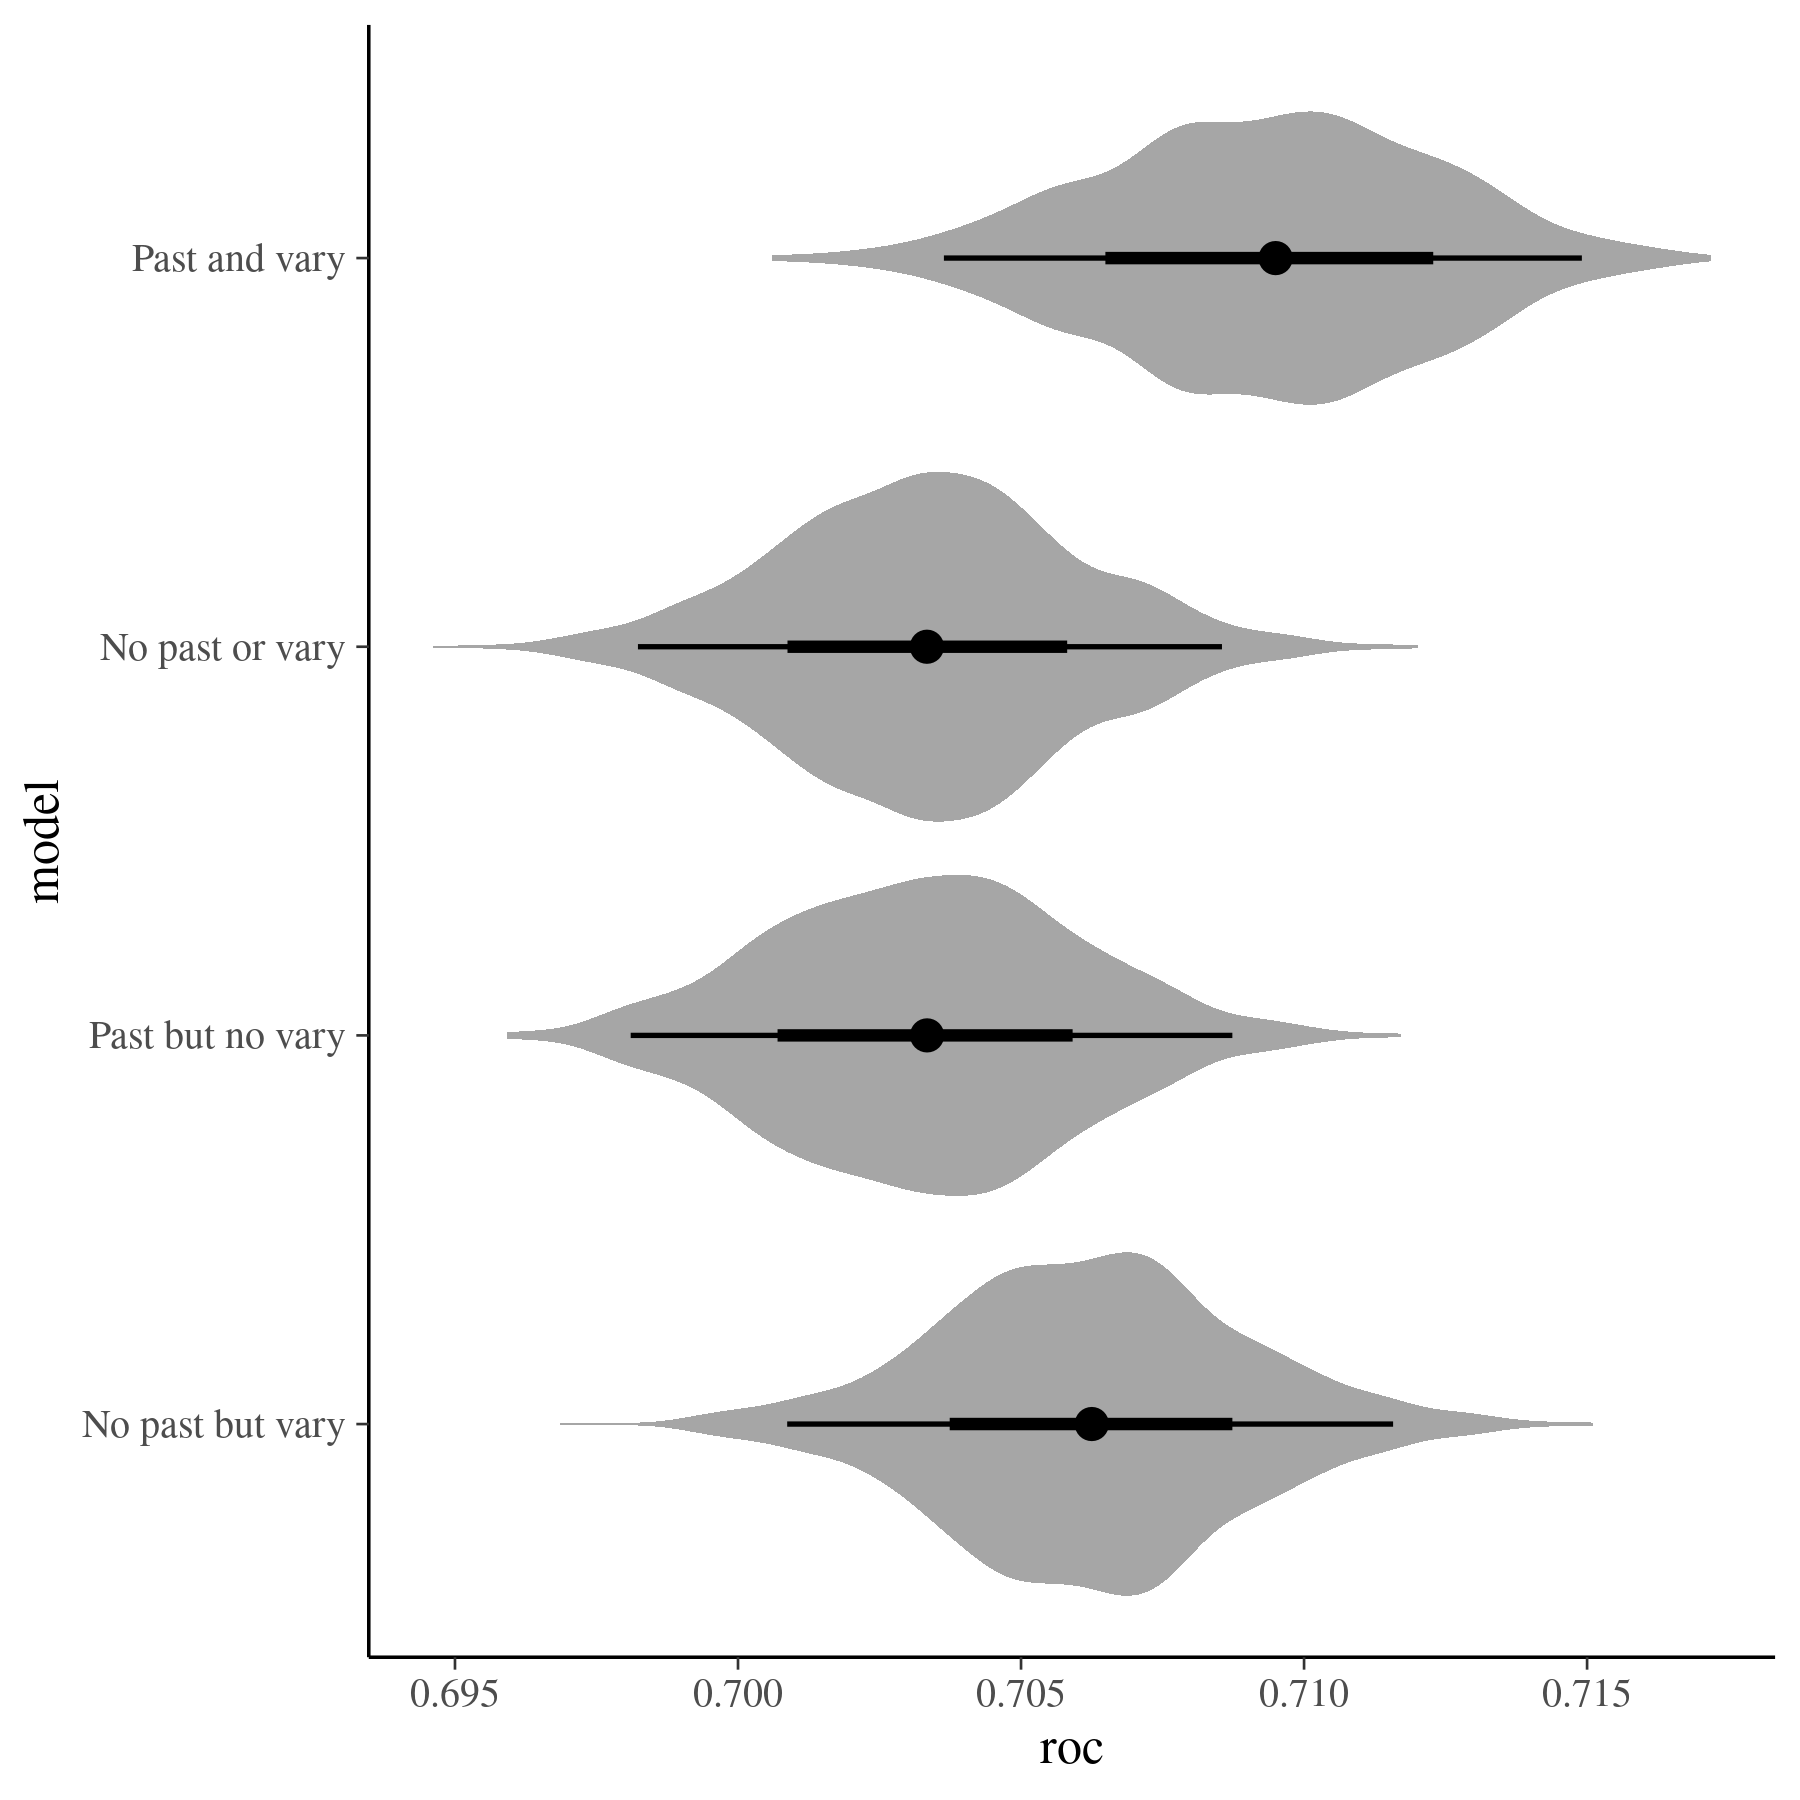
\includegraphics[width=\textwidth,height=0.5\textheight,keepaspectratio=true]{figure/roc_hist}
  \caption{Comparison of AUC estimates between the four models. These estimates are based on in-sample values. Higher values indicate greater performance.}
  \label{fig:roc_hist}
\end{figure}

Additional comparison of in-sample model performance at each of the time intervals reveals just how similar our four models are to each other (Fig. \ref{fig:roc_ts}). There are few if any obvious differences between the models in their performances.
% ROC model comparison time series
\begin{figure}[ht]
  \centering
  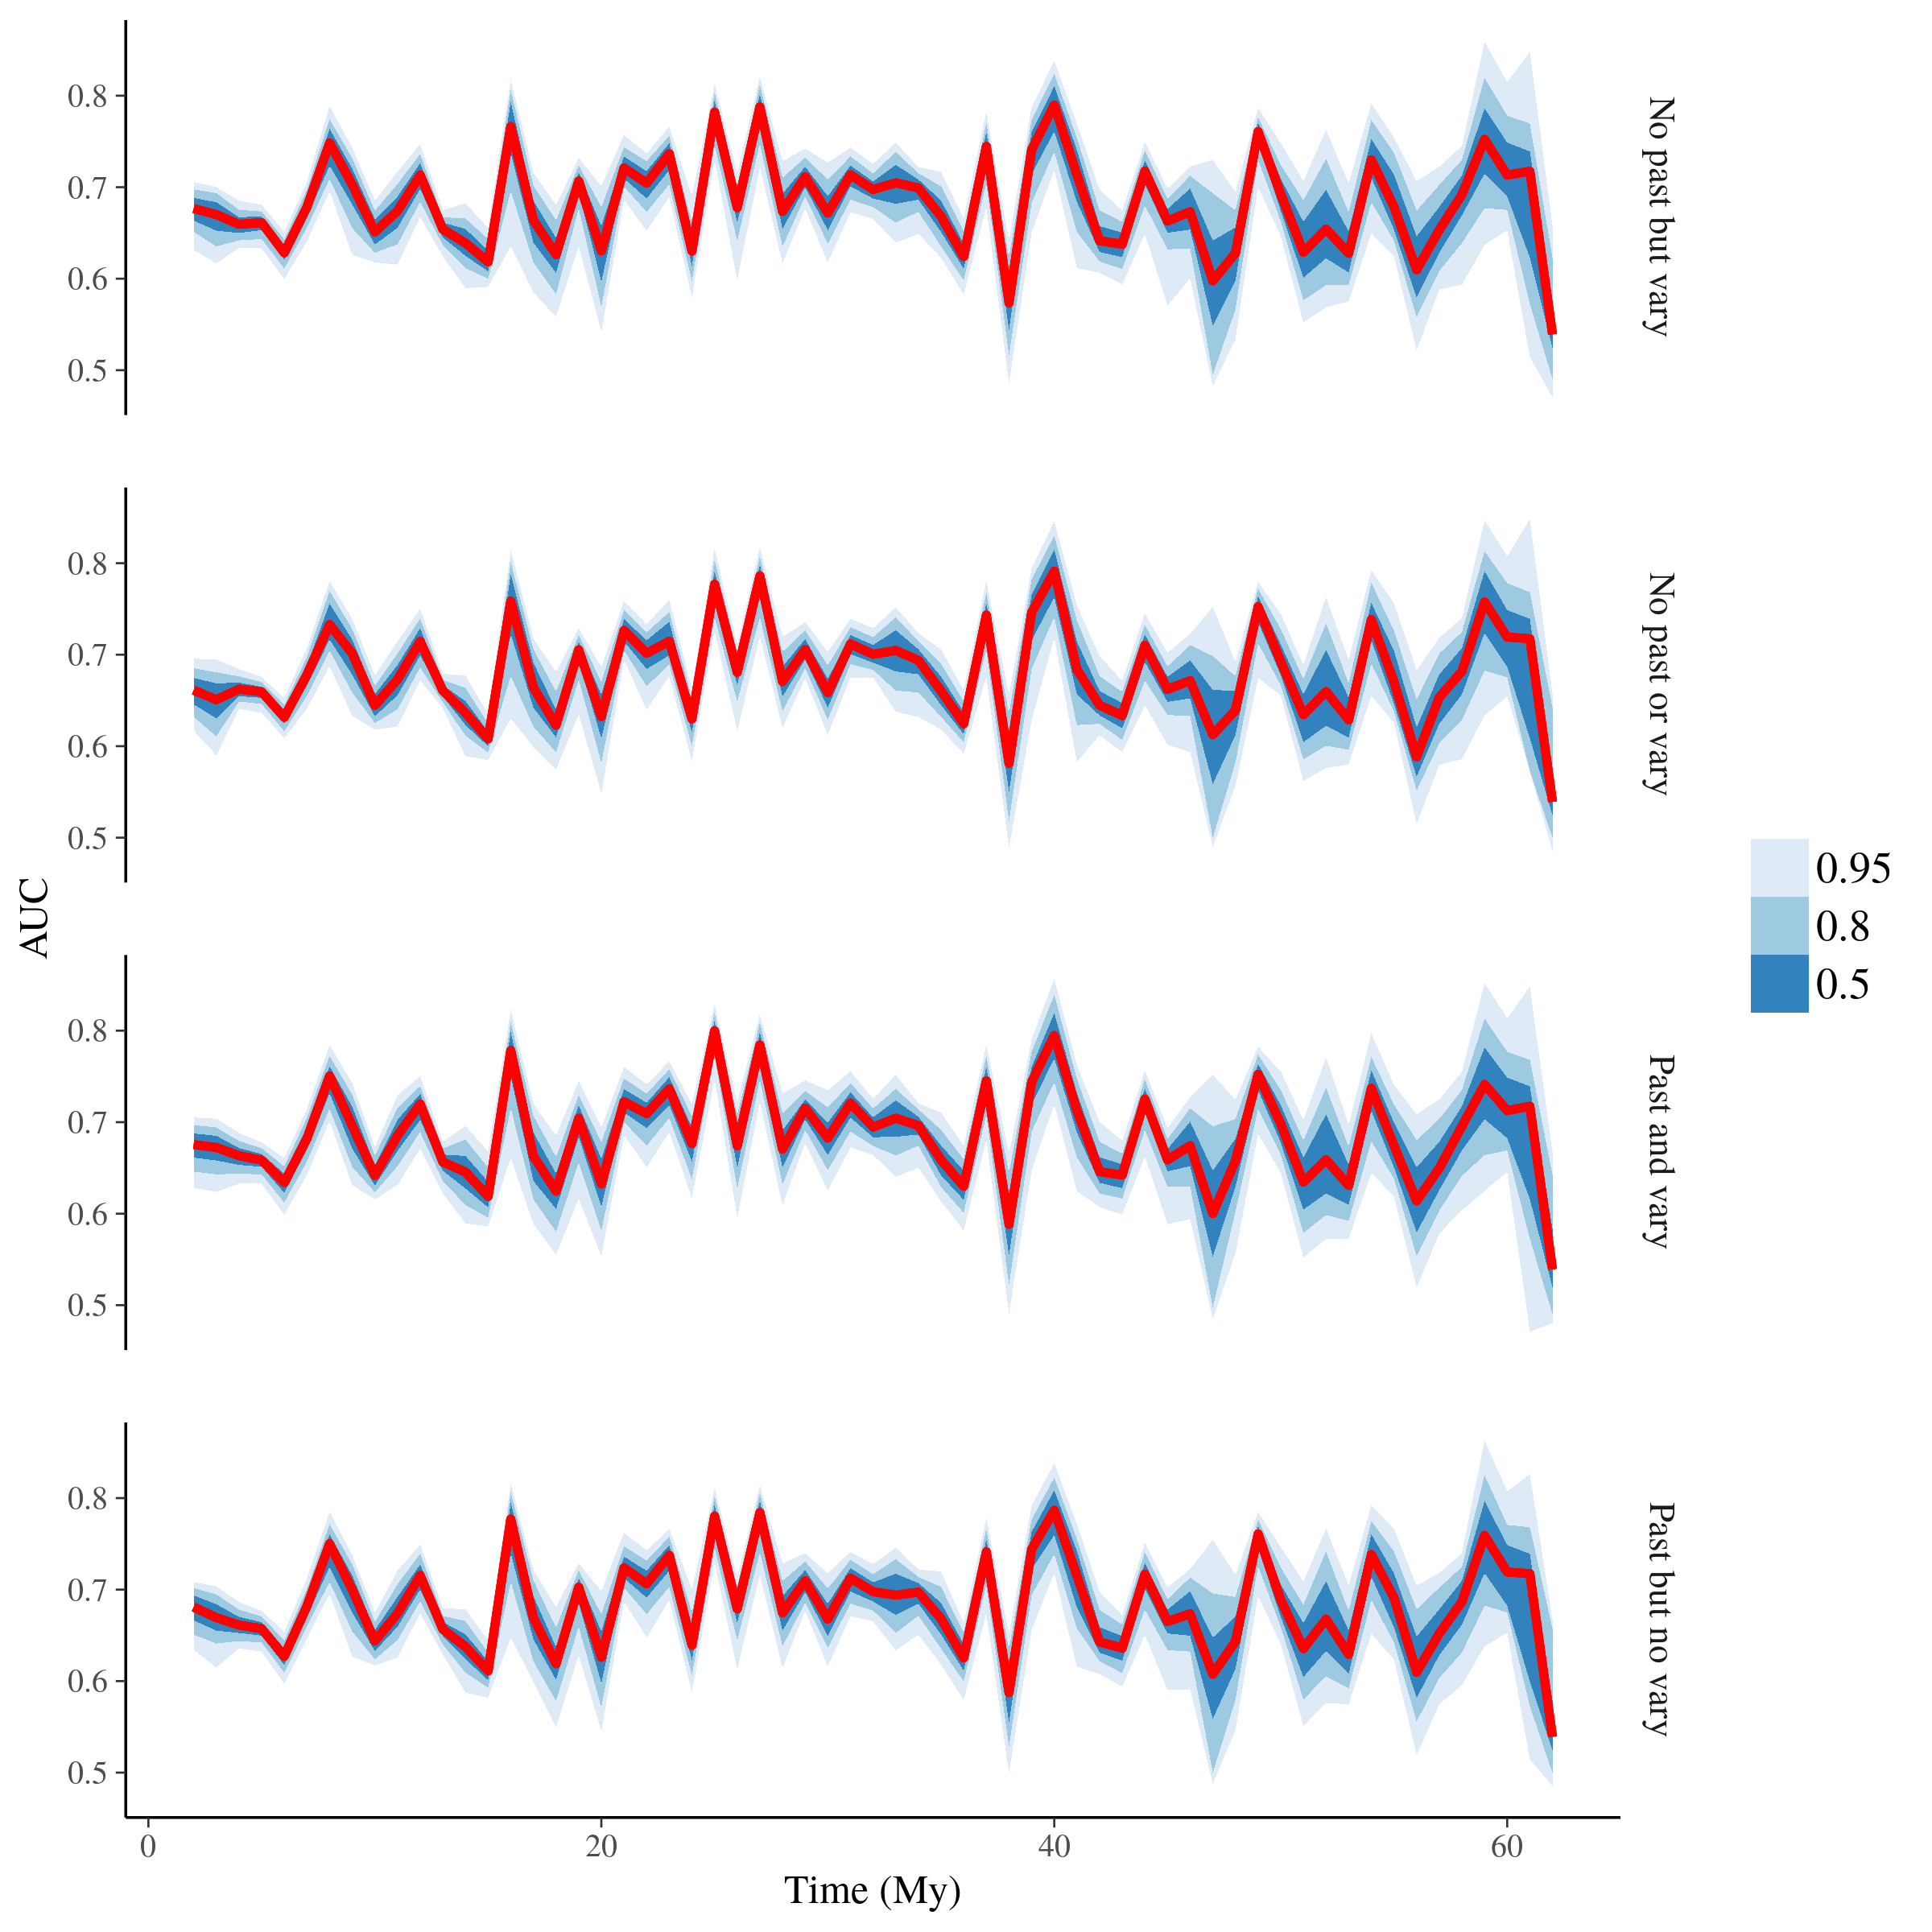
\includegraphics[width=\textwidth,height=0.5\textheight,keepaspectratio=true]{figure/roc_ts}
  \caption{Comparison of time-specific AUC values between the four models. These estimates correspond to the models ability to predict or fit that section of the data. Higher values indicate greater performance.}
  \label{fig:roc_ts}
\end{figure}

Because of the parameter rich ``past and vary'' model displays some modest improvements over the other models we choose this model for all further analysis.

\section{Cross-validation}

The approximate out-of-sample predictive performance for our selected model, as measured by AUC, is approximately identical to our in-sample performance (Fig. \ref{fig:fold_auc}). The quality of performance, however, is not great, with average out-of-sample AUC estimated to be just above 0.7 which is far from perfect. This result means that while we expect our model to yield consistent results when provided with new data, we do not expect that our predictions will be very accurate.
% ROC OOS estimate
\begin{figure}[ht]
  \centering
  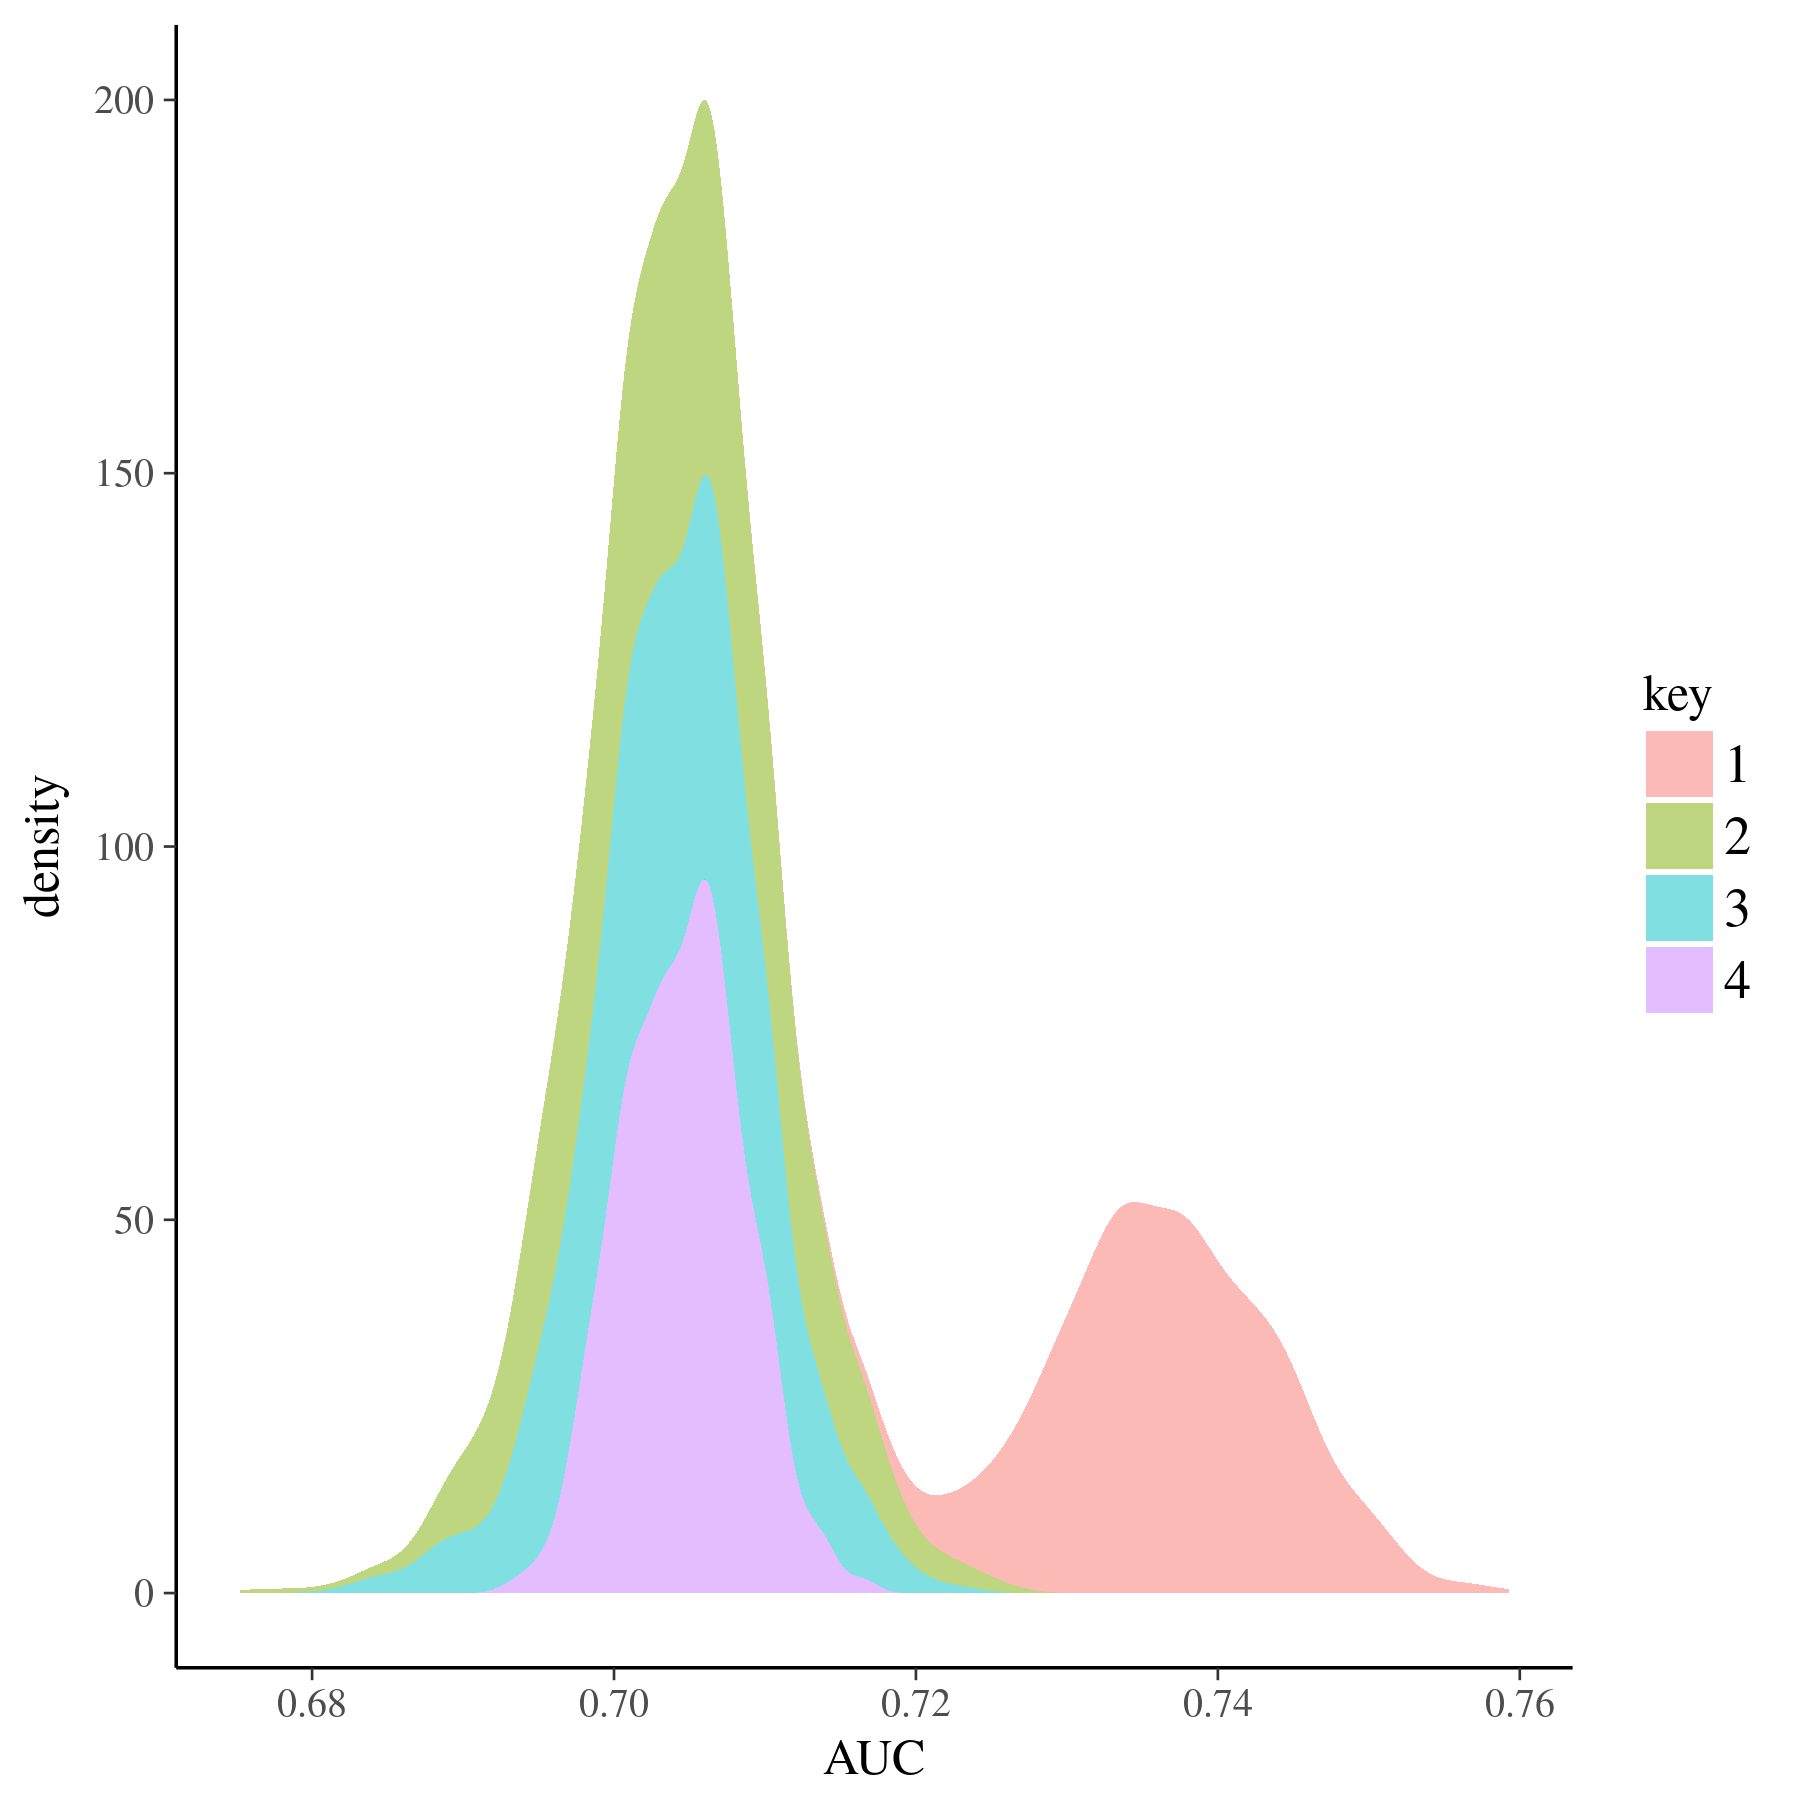
\includegraphics[width=\textwidth,height=0.5\textheight,keepaspectratio=true]{figure/fold_auc}
  \caption{Approximate out-of-sample AUC values calculated from five-fold cross-validation of the time series. The AUC estimates from each fold are labeled. Folds are numbered from oldest to youngest.}
  \label{fig:fold_auc}
\end{figure}

%When our cross-validation estimates are presented for each time interval, 
%% ROC OOS estimate time series
%\begin{figure}[ht]
%  \centering
%  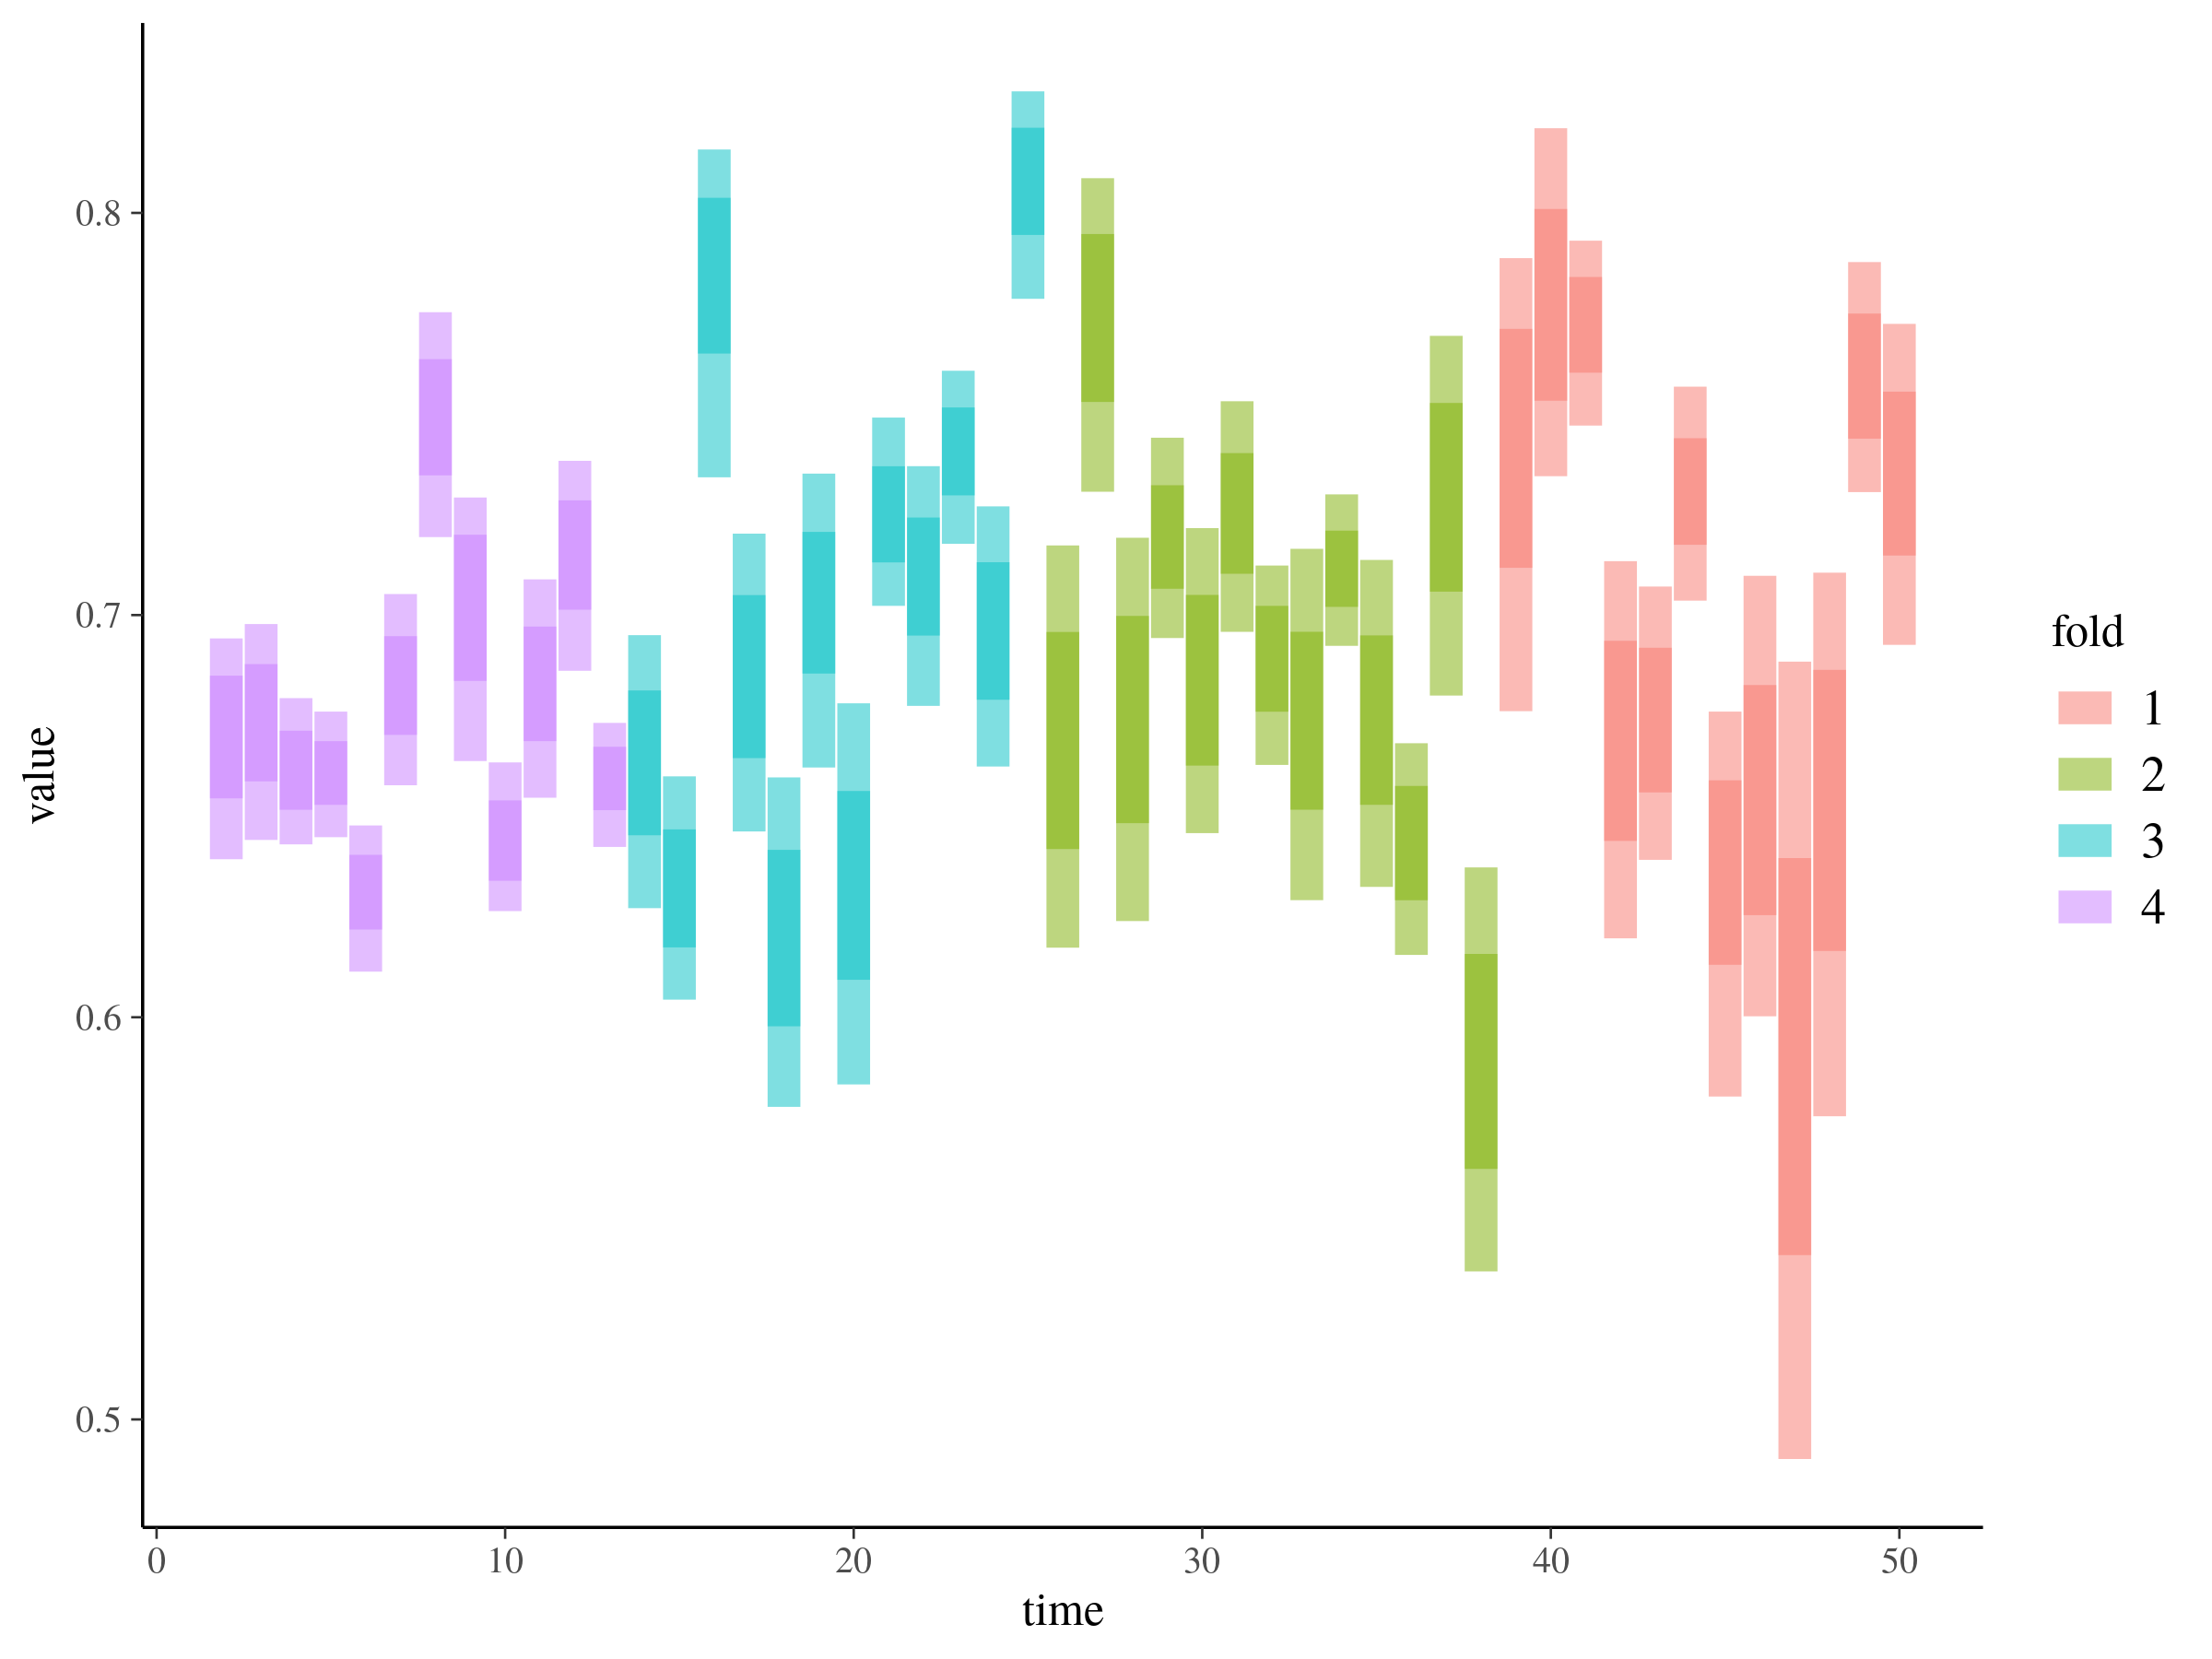
\includegraphics[width=\textwidth,height=0.5\textheight,keepaspectratio=true]{figure/fold_auc_time}
%  \caption{Approximate out-of-sample AUC values calculated for each of the My intervals using five-fold cross-validation of the time series. The AUC of the individual My intervals within each fold is plotted to highlight the heterogentity in performance within and between folds. The AUC estimates from each fold are labeled and are numbered from oldest to youngest.}
%  \label{fig:fold_auc_time}
%\end{figure}


\section{Parameter estimates}

The overall average probability of a species going extinct during any interval is very low (Fig. \ref{fig:effect_est}). This result means that even if covariate effects are very large on the log-odds scale, when compared on the probability scale will only produce a minor change in probability of extinction. This is one of the hardest parts of logistic regression for people to understand. Effect sizes are on the log-odds scale but prediction is on the probability scale. When the intercept term is very negative or positive (greater than 2), covariate effects are fighting over an increasingly small amount of probability. Logistic regressions are easiest to interpret when the intercept term is approximately 0; this is a fundamental difficulty of dealing with very uneven data sets.

As expected, a species with greater than average geographic range is expected to have a greater probability of surviving than a species with average or less than average geographic range (Fig. \ref{fig:effect_est})

We estimated an overall positive effect of the change in geographic range on extinction probability; this means that a species gaining in geographic range between that observation and their previous observed geographic range is associated with a greater extinction risk than a species which decreased in geographic range (Fig. \ref{fig:effect_est}).

We estimated an overall positive effect of both global temperature and the lag of global temperature with species extinction probability (Fig. \ref{fig:effect_est}. This type of effect means that when global temperature is above the Cenozoic average, we would expect higher than average extinction risk. Similarly, if global temperature was above the Cenozoic average in the time interval before the current one, we would also expect higher than average extinction risk. This means that during a run of above Cenozoic average global temperatures (2+ intervals) we would expect an even greater extinction risk than if just the current interval is of above average temperature.

% effects, average
\begin{figure}[ht]
  \centering
  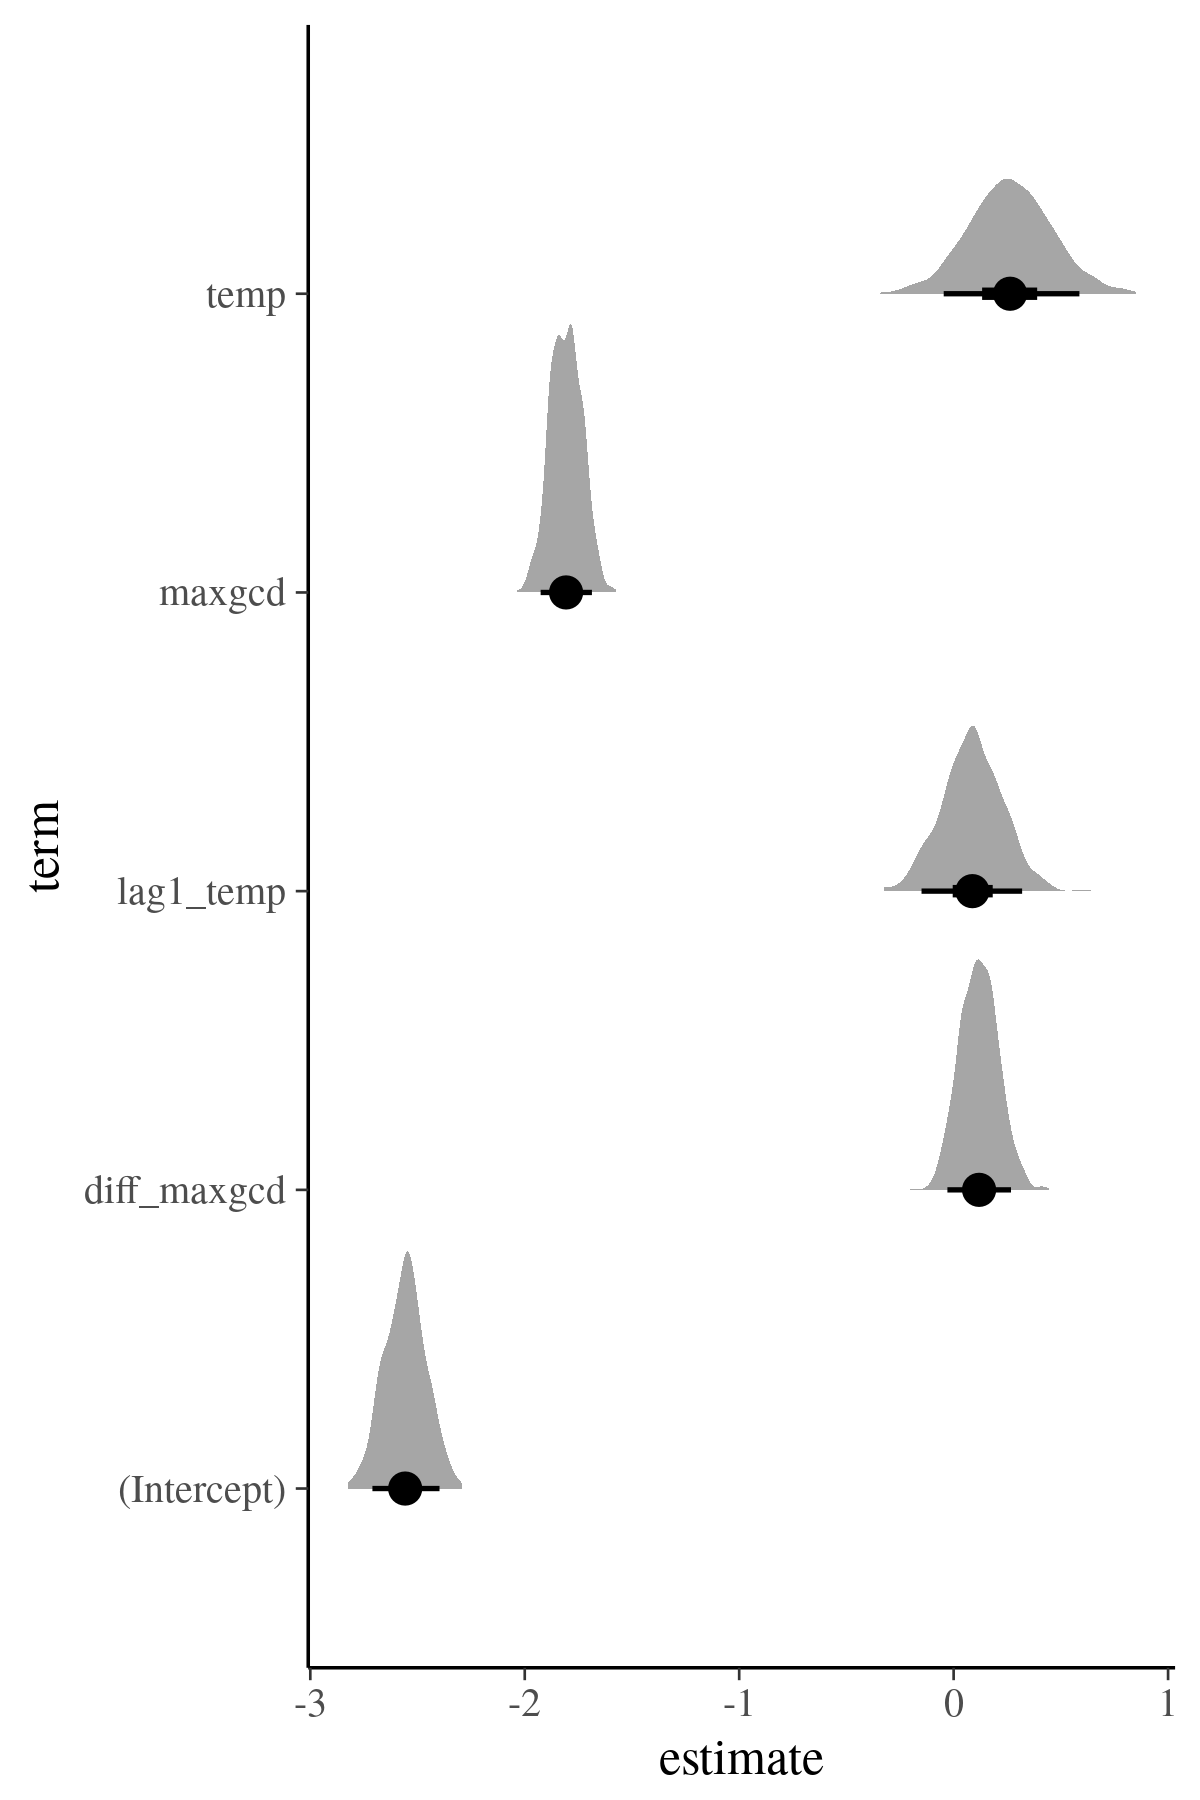
\includegraphics[width=\textwidth,height=0.5\textheight,keepaspectratio=true]{figure/effect_est}
  \caption{Estimates of the overall average covariate effects. These are averaged both over time and across phyla. The entire posterior is presented, with the median estimate labeled and 80\% credible intervals.}
  \label{fig:effect_est}
\end{figure}


The overall effect averages described above do not reflect the between time-interval variance of the effects. While the effect of geographic range has a consistent sign for the entire Cenozoic, the effects of the other covariates do not have a consistent sign (Fig. \ref{fig:effect_time_group}).

% effects, time series
\begin{figure}[ht]
  \centering
  \includegraphics[width=\textwidth,height=0.5\textheight,keepaspectratio=true]{figure/effect_time_group}
  \caption{Covariate effect estimates for the effect of geographic range and the change in geographic range for all time points and phyla. The red line corresponds to the median estimate at each time, the dark blue area corresponds to the 50\% credible interval, the medium blue the 80\% credible interval, and the light-blue the 95\% credible interval.}
  \label{fig:effect_time_group}
\end{figure}

% variance components
\begin{figure}[ht]
  \centering
  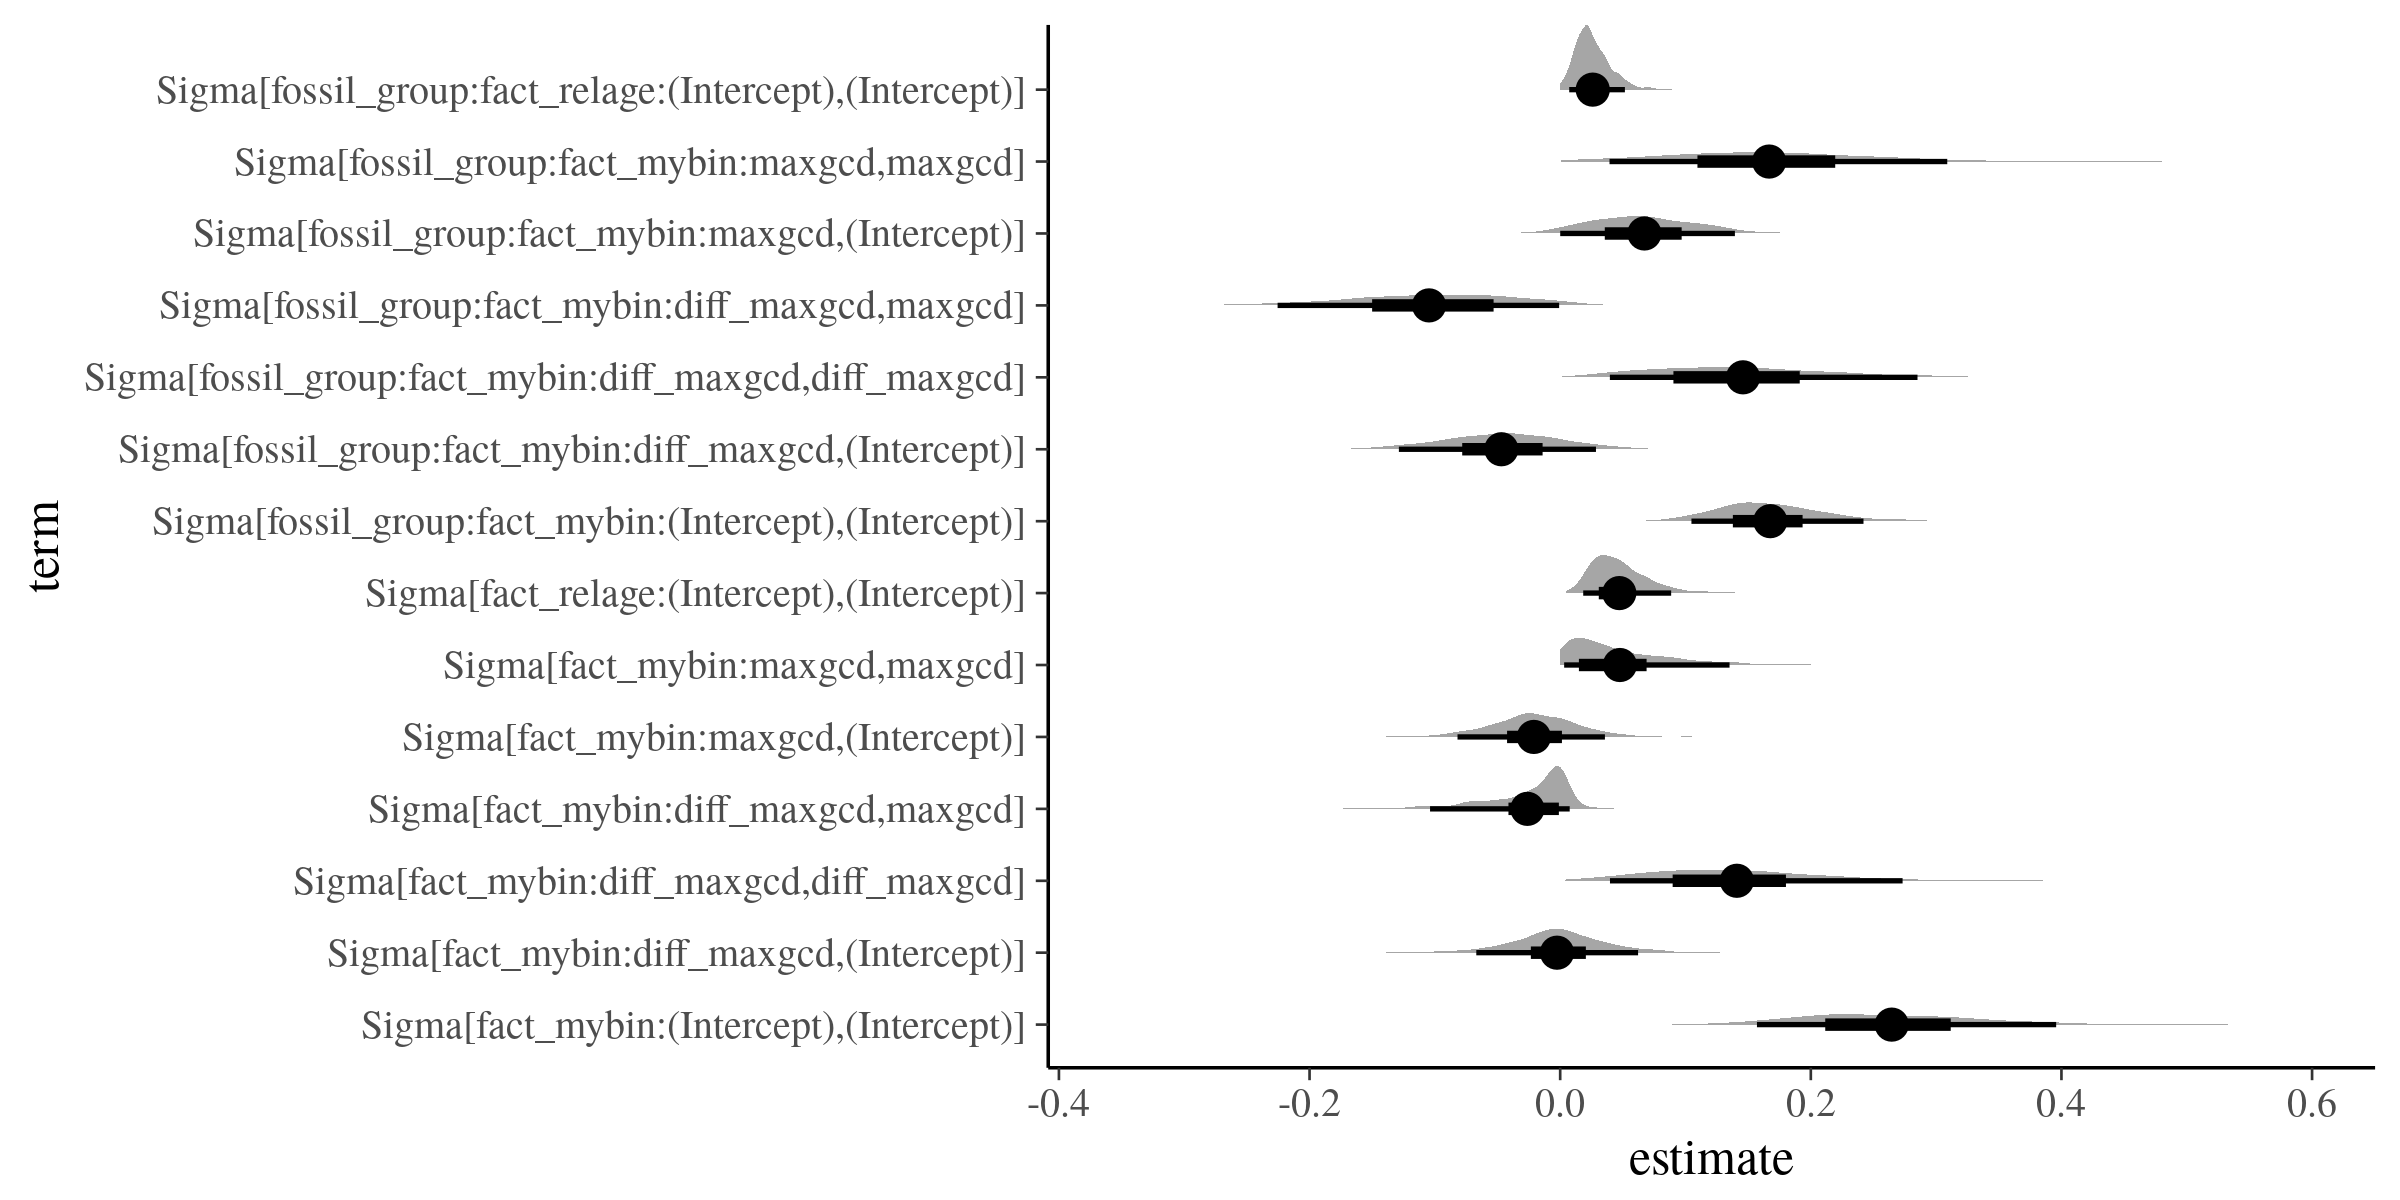
\includegraphics[width=\textwidth,height=0.5\textheight,keepaspectratio=true]{figure/variance_components}
  \caption{Contribution of multi-level components to unmodeled variance. Larger values indicate a greater contribution to overall variance. Variance components labeled as ``overall'' represent variance between grouping factors, while those labeled  ``within groups'' correspond to variance within grouping factors. If the overall component is greater than the within component, then the groupings do not structure the overall variance. If the within component is greater than the overall component, then the overall variance is structured by the groupings.}
  \label{fig:variance_components}
\end{figure}

% risk estimate compared to change in geo-range


\end{document}
